\chapter{Event selection}
The event selection extracts pairs of signals
in the data stream that have properties expected of
IBD interactions: a prompt positron annihilation
followed by a delayed neutron capture on hydrogen.
At each step in the selection, it is critical that
differences in cut efficiency between the ADs are both
minimized and quantified so that any observed near-far difference
can be justifiably attributed to oscillations.

Certain backgrounds, namely muons, PMT flashers, and accidental coincidences,
are frequent enough that their characterization, veto, and/or subtraction
are handled as part of the event selection process.
I will briefly describe these backgrounds inline
but leave detailed descriptions and studies
to the appropriate sections in \cref{ch:background}.

\section{Initial data preparation}

Before physics events are identified,
the data is cleaned in two ways.
First, cosmogenic muon events are identified
and a time window after each muon is vetoed
to allow for any spallation products or activated nuclei to decay
without contaminating the IBD signal (\cref{sec:muonveto}).
Second, occurrences of PMT light emission, known as ``flashers,''
are also vetoed and removed from the data stream (\cref{subsec:flashers}).

\section{Coincidence selection}
\label{sec:coincidence}

The first step in the event selection is
to group together signals that are close together in time
into ``coincidence groups.''
Each \SI{1}{\micro\second} triggered readout window
with reconstructed energy above \SI{1.5}{\mega\electronvolt}
is identified as an ``AD event''
and is a potential coincidence candidate.
Because of the nonzero length of the readout window,
AD events occurring closer together than \SI{1}{\micro\second}
are not necessarily separate physical events.
Consequently, during the coincidence grouping process,
the coincidence search window begins \SI{1}{\micro\second}
after the initial AD event.
Coincidence groups are constructed by repeating the following steps
until the data file is exhausted:

\begin{enumerate}
    \item Find the next AD event.
        This AD event will be the ``prompt'' event of the coincidence group.
    \item Find all subsequent AD events within the desired coincidence time \tc.
        If a muon event is encountered within \tc,
        veto the entire coincidence group starting with the prompt event.
        (This additional vetoed time is accounted for in the muon veto efficiency.)
    \item Group these events together with the prompt event
        to form the coincidence group.
    \item Skip to the next AD event that is not part of the coincidence group.
\end{enumerate}

\begin{figure}
    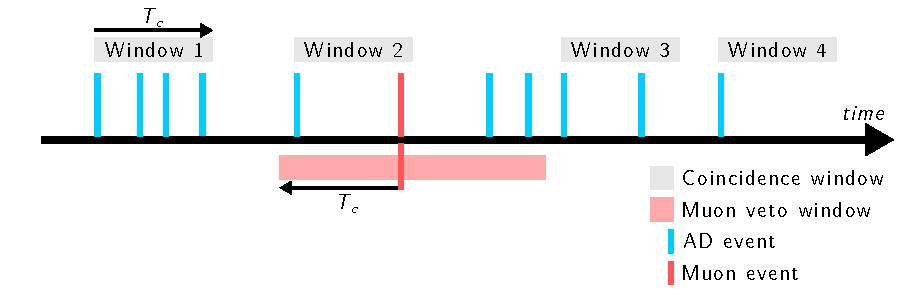
\includegraphics{ch_event_selection/timeline_examples}
    \caption{
        An example timeline showing how coincidence groups are created,
        and how they interact with muons and muon veto windows.
        This illustration does not show the \SI{1}{\micro\second} gap
        at the start of each coincidence window.
        Windows 1, 3, and 4 are valid coincidence groups,
        while Window 2 is vetoed by the muon event.
    }
    \label{fig:timeline_examples}
\end{figure}

Because of the initial \SI{1}{\micro\second} gap,
the actual time interval covered by any given coincidence window is
$\tc - \SI{1}{\micro\second}$.
This analysis uses a coincidence search window of $\tc = \SI{1.5}{\milli\second}$.

The total number of AD events in the group
is the multiplicity of the group.
A coincidence group with multiplicity $n$ is also referred to
as an \fold{n} coincidence.
In Window 1 of \cref{fig:timeline_examples},
the first AD event starts a new coincidence window
that includes three other AD events,
resulting in a coincidence group of multiplicity 4, or a \fold{4} coincidence.

If a muon event occurs within a coincidence window,
then that coincidence window is vetoed.
In other words, every muon has an implicit veto window
that forbids prompt events within \tc{} of the muon.
This is demonstrated by Window 2 of \cref{fig:timeline_examples}.
Note that if the prompt event occurs earlier than \tc{} before a muon,
then subsequent events within the coincidence window
are allowed to occur inside of the implicit muon veto window.
Only prompt events are vetoed by the implicit veto window.

The veto window after a muon also impacts the way that
coincidence windows are formed.
Window 3 of \cref{fig:timeline_examples} shows a coincidence window
whose prompt event is preceded by other recent AD events.
However, those AD events fall within the previous muon veto window,
so they are ignored for the purposes of forming coincidence groups.

If a prompt event has no subsequent AD events within \tc, it is
still a valid group, and is referred to as a \fold{1} coincidence.
Note that \fold{1} coincidences are somewhat but not strictly isolated
from other AD events.
Certainly there are no other AD events
within \tc{} \textit{after} the prompt event,
but there may be a \textit{preceding} AD event within \tc{}
if that event is part of a coincidence window
which ends before the prompt event in question.
Window 4 of \cref{fig:timeline_examples} demonstrates this property:
there are no other AD events within Window 4,
but there is a previous AD event within \tc{} of the start of Window 4.
Given the event rates at Daya Bay, this only happens in $\sim10^{-4}$
of single events.
This probability is derived in \cref{ap:singlesformula} as $P_b$.

\newcommand{\adheight}{0.23\textheight}
\newcommand{\adspacing}{1cm}
\newcommand{\adinclude}[1]{
    \includegraphics[height=\adheight, trim={0 0 0 1cm}, clip]{#1}
}
\newcommand{\adgrid}[3]{
    \begin{figure}
        \centering
        \adinclude{#3_EH1_AD1}
        \hspace{\adspacing}
        \adinclude{#3_EH1_AD2}\\
        \adinclude{#3_EH2_AD1}
        \hspace{\adspacing}
        \adinclude{#3_EH2_AD2}\\
        \adinclude{#3_EH3_AD1}
        \hspace{\adspacing}
        \adinclude{#3_EH3_AD2}\\
        \adinclude{#3_EH3_AD3}
        \hspace{\adspacing}
        \adinclude{#3_EH3_AD4}
        \caption{#1}
        \label{#2}
    \end{figure}
}

\adgrid{All double coincidences found using $\tc=\SI{1.5}{\milli\second}$}{fig:double_coinc_raw}{ch_event_selection/double_coincs}

Once the coincidence groups have been constructed,
the set of \fold{2} coincidences can be identified as
the preliminary set of IBD candidates,
albeit with background still present.
\Cref{fig:double_coinc_raw} shows the prompt and delayed energy
of all \fold{2} coincidences identified in EH1-AD1 and EH3-AD1
as representatives of the near and far sites.
These plots clearly show the nGd events
at delayed energy values near \SI{8}{\mev}.
The nH events are visible as the narrow band at
delayed energies near \SI{2.2}{\mev}
and prompt energies of \SIrange{4}{7}{\mev}.
At prompt energies less than \SI{3.5}{\mev} or greater than \SI{7}{\mev}
these signal events are overwhelmed by the accidental background,
which is characterized in these plots by the 4-point square at both prompt and
delayed energies of \SIlist{1.5;3.25}{\mev}.

The \fold{1} coincidences can be identified as a subset
of the uncorrelated events, mostly radioactive decays,
that are also present in the data stream.
However, not all uncorrelated events end up in \fold{1} coincidences.
Sometimes an uncorrelated event will occur in close proximity to
a true IBD prompt-delayed pair, creating a \fold{3} coincidence.
These high-multiplicity coincidence groups are vetoed
with a small loss of efficiency.
More concerning is when two uncorrelated events
randomly occur in close proximity to each other,
creating a \fold{2} coincidence group that passes the high-multiplicity veto.
These so-called ``accidental'' coincidences
constitute the largest background within the set of \fold{2} coincidences
(\cref{subsec:acc}).
The distance, time and energy cuts described below
are all motivated in large part by the need to reduce the accidental background.

\section{Distance and time cuts}

The distance and time distributions between prompt and delayed AD events
are different depending on the physical process producing those AD event pairs.
For example, the neutron produced during an IBD interaction
scatters within the liquid scintillator until being captured
by a hydrogen nucleus,
traveling a characteristic distance over a characteristic time.
On the other hand, two uncorrelated events have, by definition,
no particular connection between their physical locations
or their timings.

In practice, the characteristic distance for a neutron capture on hydrogen
is approximately \SI{200}{\milli\meter},
and the characteristic time delay is \SI{200}{\micro\second}.
For accidental coincidences, the characteristic distance is
the length scale of the AD, approximately \SI{3000}{\milli\meter},
and the time delay has a flat probability distribution
on the time scale used for the coincidence window ($\tc = \SI{1.5}{\milli\second}$).

\adgrid{Distribution of coincidence distance and coincidence
time}{fig:dr_vs_dt}{ch_event_selection/dr_vs_dt}

\Cref{fig:dr_vs_dt} shows the distribution of
coincidence distance and coincidence time
for the subset of \fold{2} coincidences with
relatively small coincidence distances and times
of less than \SI{1000}{\milli\meter} and \SI{600}{\micro\second},
respectively.
Correlated events are grouped at the lowest
coincidence times and distances,
although there is a visible tail in both dimensions.
The rest of the events distributed with relatively uniform density
across the plot are accidental background from uncorrelated events.
This plot was used to determine the distance and time cut
by drawing a line from \SI{800}{\milli\meter} at $0$ time
to \SI{480}{\micro\second} at $0$ distance.
This line rather effectively separates the higher-density region
of correlated events from the uniform density region of accidental background.
This cut is known as the DT cut and the line determining the cut has the equation

\begin{equation}
    \text{DT} = \Delta r + v_0 \Delta t < \SI{800}{\milli\meter},
\end{equation}
where $v_0 = \frac{\SI{1000}{\milli\meter}}{\SI{600}{\micro\second}}$.
Note that the quantity DT is not D times T,
nor should it be confused the differential $dt$.
\Cref{fig:after_DT_cut} shows the individual AD spectra
after applying the DT cut.
As expected, the accidental background present
in the low-prompt-energy and low-delayed-energy corner is much reduced.
The neutron capture on hydrogen events now stand out much better
against the accidental background.

\adgrid{Prompt-delayed energy spectra after applying
the DT cut}{fig:after_DT_cut}{ch_event_selection/post_DT_cut}

Applying the DT cut rejects the vast majority of accidental events
at a loss of approximately \SI{30}{\percent} of real IBDs.
The efficiency is measured after subtracting the accidental background
(\cref{subsec:acc})
by comparing the number of \fold{2} coincidences that pass the energy cuts and the DT cut
with the number of \fold{2} coincidences that pass the energy cuts
and a significantly relaxed DT cut of \SI{3000}{\milli\meter}:

\begin{equation}
    \varepsilon_{\text{DT}} = \frac{N(\text{DT} < \SI{800}{\milli\meter})}{
    N(\text{DT} < \SI{3000}{\milli\meter})}
\end{equation}
As the histograms in \cref{fig:ed_DT_sub} show,
negligibly few IBDs have a DT value anywhere close to \SI{3000}{\milli\meter},
so $\varepsilon_{\text{DT}}$ closely approximates the true efficiency.
The DT cut efficiency for each AD is shown in \cref{fig:DT_eff}.

\begin{figure}
    \centering
    \includegraphics[width=0.49\textwidth, trim={0 0 0 1cm}, clip]{%
        ch_event_selection/ed_DT_sub_EH1_AD1%
    }
    \includegraphics[width=0.49\textwidth, trim={0 0 0 1cm}, clip]{%
        ch_event_selection/ed_DT_sub_EH2_AD1%
    } \\
    \includegraphics[width=0.49\textwidth, trim={0 0 0 1cm}, clip]{%
        ch_event_selection/ed_DT_sub_EH3_AD1%
    }
    \caption{
        The accidentals-subtracted distribution of
        delayed energy and DT value, used to compute $\varepsilon_{\text{DT}}$.
        The green (solid) box shows the events included in the DT cut.
        The black (dashed) box shows the events excluded by the DT cut.
        The large fluctuations at high DT are due to the statistics
        of subtracting two almost-equal large numbers as part of the
        background subtraction procedure.
    }
    \label{fig:ed_DT_sub}
\end{figure}

\begin{figure}
    \centering
    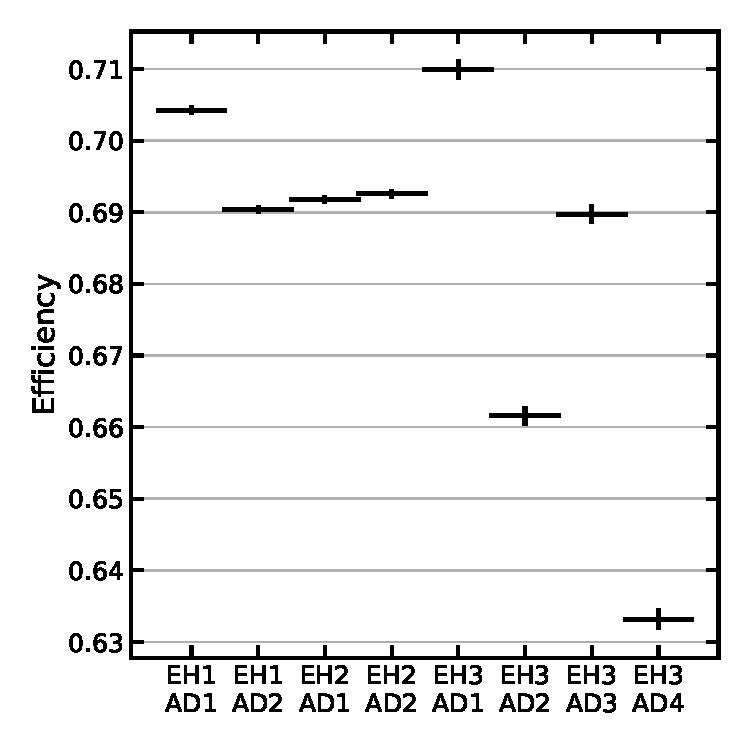
\includegraphics[height=0.4\textheight]{plot_diagnostics/distance_time_cut_efficiency}
    \caption{The DT cut efficiency for each AD. Error bars are statistical.}
    \label{fig:DT_eff}
\end{figure}

The AD-uncorrelated uncertainty for the efficiency
is determined from the data by examining the variation
in measured efficiency between the 4 near-hall ADs.
The far-hall ADs are excluded because
their statistical uncertainties are much larger than the
near-hall AD variation.
The AD-uncorrelated uncertainty of the DT cut efficiency
is the half-range of the near-hall efficiencies: \num{0.0016} (absolute),
or approximately \SI{0.23}{\percent} (relative).

\section{Energy cuts}

\subsection{Prompt energy}
The prompt energy lower bound of \SI{1.5}{\mev}
is chosen to exclude a substantial fraction
of the low-energy uncorrelated events from radioactive decays.
In particular, the electron capture process
${}^{40}\text{K} \to {}^{40}\text{Ar} + \nu_e + \gamma$
releases a $\gamma$ ray with energy \SI{1.46}{\mev}.
The high-energy tail of this interaction is visible in the prompt-delayed spectra
(\cref{fig:double_coinc_raw}) as an elevated bin content
along both the horizontal and vertical axes from \SIrange{1.5}{3}{\mev}.

\begin{figure}
    \centering
    \includegraphics[width=0.6\textwidth, trim={0, 1.5cm, 0, 0}, clip]{%
        ch_event_selection/prompt_energy_mc%
    }
    \caption{The spectrum of reconstructed energy for IBD prompt events
        in the Monte Carlo study used to compute the prompt energy efficiency
    and AD-uncorrelated uncertainty}
    \label{fig:prompt_eff_mc}
\end{figure}
The nominal efficiency of the prompt energy cut is estimated using Monte Carlo.
The spectrum of ``true'' IBD prompt event reconstructed energy
is shown in \cref{fig:prompt_eff_mc}.
Only events with energy above \SI{1.5}{\mev} on this histogram
are included in the IBD event selection.

%TODO figure
However, because of the energy dependence of the \nuebar{} oscillations,
a different fraction of \nuebar{} will pass this cut
depending on the baseline between the reactor and the AD.
For example, at shorter baselines, low-energy \nuebar{}
are more likely to oscillate to other flavors, so that at the near halls,
there are fewer IBD events missed by the prompt energy cut,
thus raising the efficiency of the cut.
At the oscillation maximum, though, medium-energy \nuebar{},
around \SIrange{2}{3}{\mev}, are most likely to oscillate.
So a smaller fraction of IBDs will pass the cut,
and the efficiency will be lower.

Corrections for each AD--reactor pair should be computed
and weighted to arrive at each AD's final prompt energy efficiency.
Since the corrections to the efficiency depend on
the amplitude of \nuebar{} oscillations, they rely on knowledge of \thetaot.
(For example, there would be no corrections at all if \thetaot{} were $0$.)
To compute accurate corrections and, more importantly, an accurate value
for \thetaot{}, an iterative process is used.
Initially, no baseline-dependent correction is used and
a value for \thetaot{} is obtained.
That initial \thetaot{} is then used to compute baseline-dependent corrections,
and the updated efficiencies are used to compute an updated value for \thetaot{}.
This process is repeated until the \thetaot{} result converges.
%TODO figure

The AD-uncorrelated uncertainty for the prompt energy lower bound
is dominated by differences in the energy scale between ADs.
Based on the analysis of the delayed energy spectrum in each AD
reported in \cref{subsec:delayed}, the energy scale
varies by less than \SI{0.5}{\percent} between ADs.
By applying a \SI{+-0.5}{\percent} variation to
the event energy in the Monte Carlo dataset as visualized in \cref{fig:prompt_eff_mc},
the impact of the energy scale differences can be propagated
to the prompt energy efficiency.
The impact, and therefore the relative uncertainty on
the prompt energy efficiency, is observed to be \SI{0.1}{\percent}.

There is also a \SI{12}{\mega\electronvolt} upper bound for the prompt energy.
The reactor \nuebar{} spectrum falls steeply above \SI{8}{\mev},
so this cut is determined to have \SI{100}{\percent} efficiency.

\subsection{Delayed energy}
\label{subsec:delayed}

Neutron capture on hydrogen releases a (monoenergetic)
\SI{2.22}{\mev} $\gamma$-ray,
which means the cut values can be tuned to a narrow energy region
around that value.
However, while the prompt IBD positron essentially never escapes
from the liquid scintillator sensitive volume,
$\gamma$'s do regularly escape (a few percent of the time),
depositing less than their full energy in the liquid scintillator.
Both the tuning of the energy cut values
and the fraction of escaping $\gamma$'s are sensitive to
small variations in the geometry of the AD, energy reconstruction,
and scattering properties of $\gamma$'s in
both liquid scintillator and in acrylic.

The delayed energy cut bounds are identified based on
functional fits to each AD's delayed energy spectrum.
Specifically, the spectrum is generated by first applying
the prompt energy cut and DT cut,
then statistically subtracting the accidental background (\cref{subsec:acc}).
Although the resulting spectrum still has some background,
the only remaining background processes also involve
neutron capture on hydrogen, and contribute to the same spectral shape
as the signal IBD process.

Each spectrum is fit with the calorimeter function, which models
a calorimetric response to a monoenergetic process with ``true''
energy $\mu$.
The modeled detector has an intrinsic and energy resolution $\sigma$
which applies a Gaussian smearing to the deposited energy.
($\sigma$ itself is independent of energy.)
While many events in this model deposit all of their energy into
the calorimeter, some events partially leak out.
The fraction of events that deposit their full energy in the detector
is referred to as the peak fraction $\alpha$.
The energy leakage is modeled as an exponential distribution
with characteristic energy scale (or ``tail slope'') $\lambda$.
The fit function itself is derived by starting with
the unsmeared model:

\begin{equation*}
    f_{unsmeared}(E) =
    \begin{cases}
        \alpha\delta(E-\mu) + (1-\alpha)\lambda e^{\lambda E}
        & 0 < E \leq \mu \\
        0 & E > \mu
    \end{cases}
\end{equation*}
This function is then convolved with a Gaussian
of width $\sigma$.

\begin{align*}
    f_{cal}    &= f_{unsmeared} \otimes \text{Gaussian} \\
    f_{cal}(E) &= \int_0^\mu dE' f_{unsmeared}(E') \cdot \text{Gaussian}(E'-E; \mu) \\
               &= \frac{1}{\sigma\sqrt{2\pi}}
               \left[
                   \alpha\int_0^\mu dE' e^{-\frac{(E'-E)^2}{2\sigma^2}} \delta(E'-\mu)
                   + (1-\alpha)\int_0^\mu dE' e^{-\frac{(E'-E)^2}{2\sigma^2}}
                   \lambda e^{\lambda E'}
               \right] \\
               &= \alpha\frac{1}{\sigma\sqrt{2\pi}}e^{-\frac{(E-\mu)^2}{2\sigma^2}}
               + (1-\alpha)
               \frac{\lambda e^{\sigma^2\lambda^2+2\lambda E}}{e^{\lambda\mu}-1}
               \left[
                   \text{erf}
                   \left(
                       \frac{\mu-E-\sigma^2\lambda}{\sigma\sqrt{2}}
                   \right)
                   + \text{erf}
                   \left(
                       \frac{E + \sigma^2\lambda}{\sigma\sqrt{2}}
                   \right)
               \right]
\end{align*}
The entire result is normalized to unity
but can be scaled by an overall normalization $N$.

\adgrid{Delayed energy fits using the calorimeter function}{fig:delayed_fits}{%
    ch_event_selection/delayed_fit%
}

\begin{figure}
    \centering
    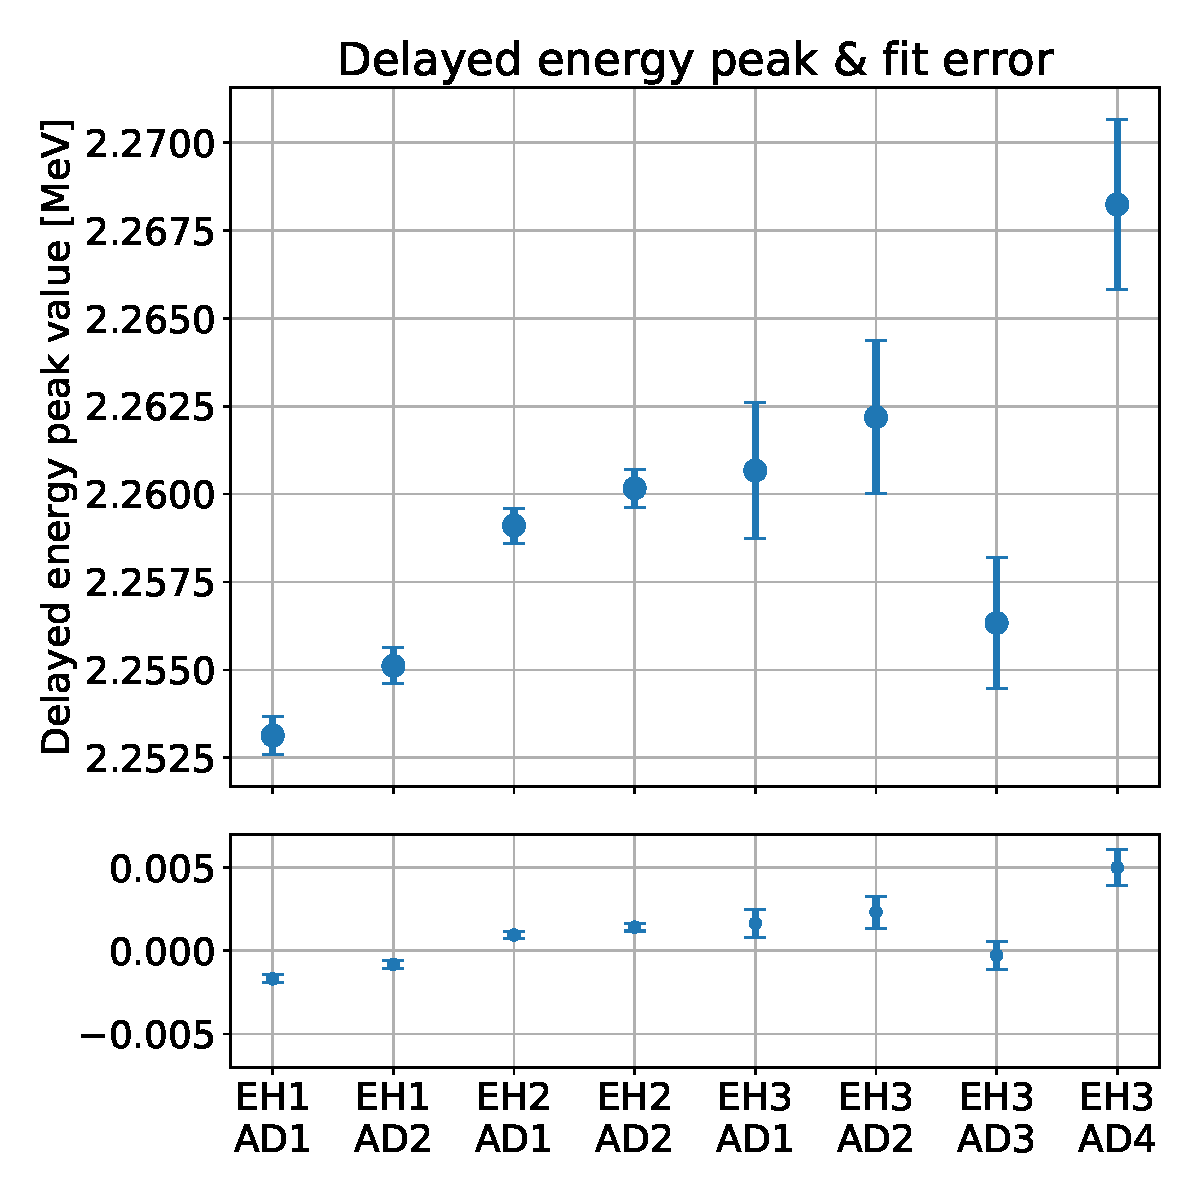
\includegraphics[height=0.33\textheight]{plot_diagnostics/delayed_energy_peak.pdf}
    \vspace{0.5cm}\hspace{0.5cm}
    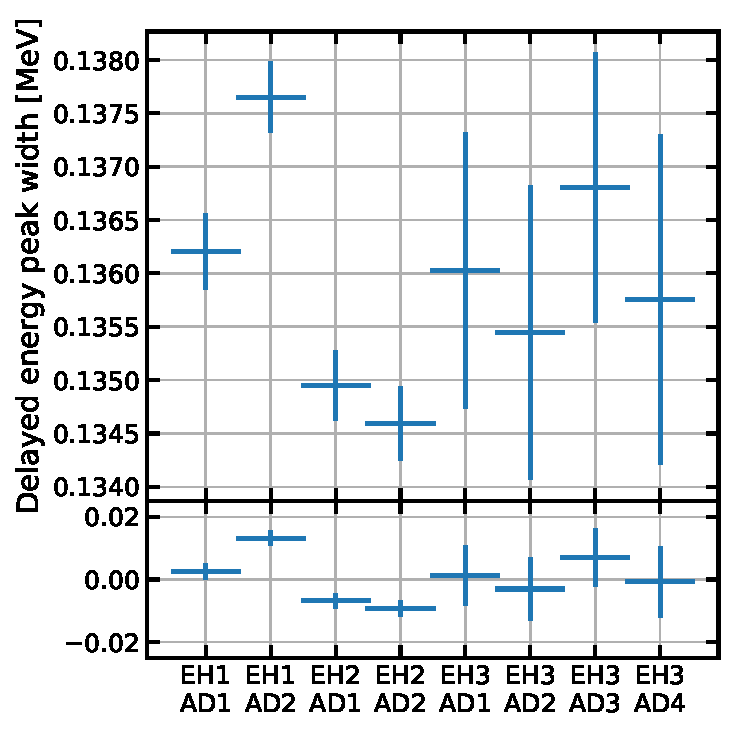
\includegraphics[height=0.33\textheight]{plot_diagnostics/delayed_energy_width.pdf}\\
    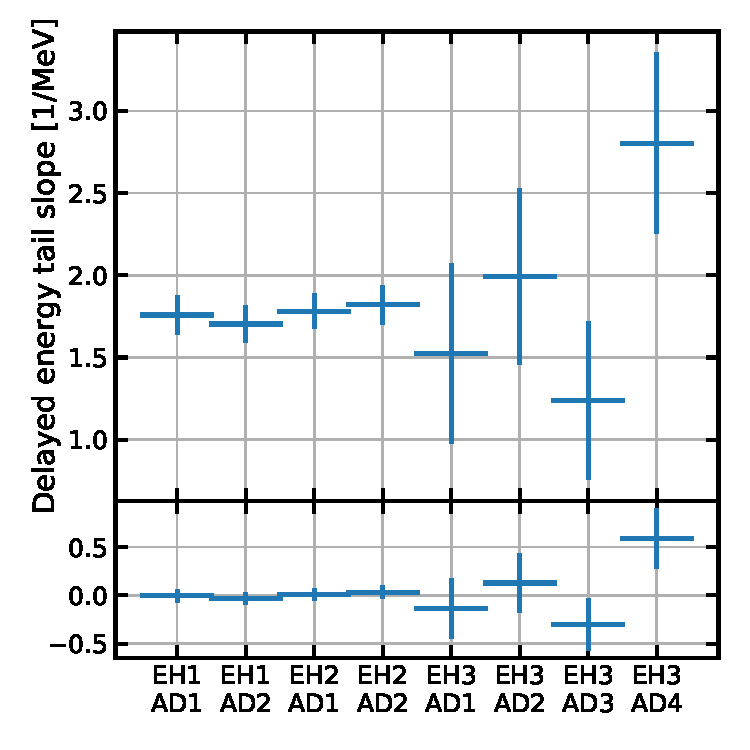
\includegraphics[height=0.33\textheight]{plot_diagnostics/delayed_energy_expo_scale.pdf}
    \hspace{0.5cm}
    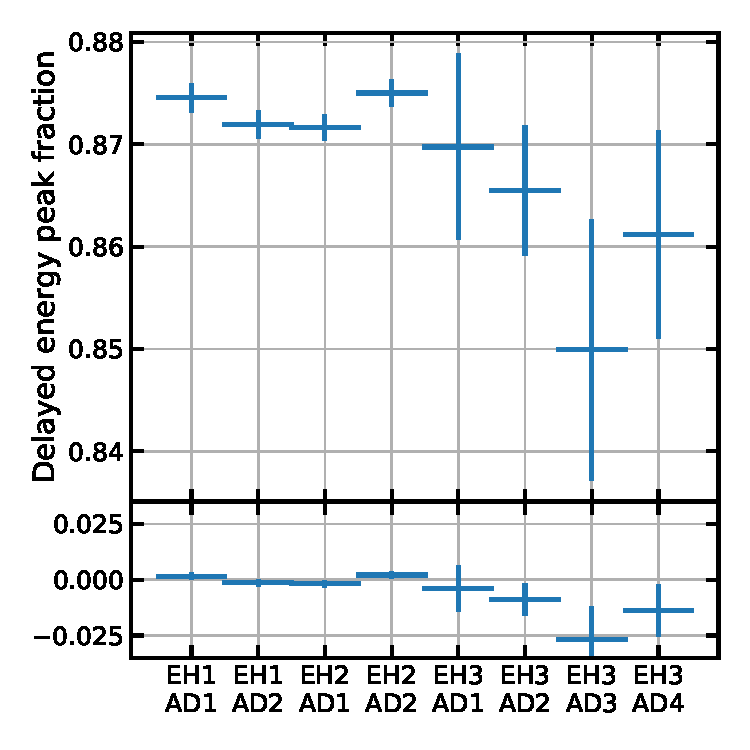
\includegraphics[height=0.33\textheight]{plot_diagnostics/delayed_energy_peak_frac.pdf}\\
    \caption{
        Fit parameters for each AD.
        Error bars represent fit errors.
        The smaller plots show the relative deviation of each AD's value
        from the average value of the 4 near-hall ADs.
    }

    \label{fig:delayed_fit_parameters}
\end{figure}

\begin{table}[ht]
    \centering
    \begin{tabular}[t]{lllll}
        \hline
        & Peak energy [\si{\mev}]
        & Width [\si{\mev}]
        & Tail slope [\si{\per\mev}]
        & Peak fraction \\
        \hline
        EH1-AD1 & \num{2.2531} & \num{0.1365} & \num{1.6893} & \num{0.8683}\\
        EH1-AD2 & \num{2.2551} & \num{0.1380} & \num{1.6247} & \num{0.8666}\\
        EH2-AD1 & \num{2.2591} & \num{0.1351} & \num{1.7212} & \num{0.8663}\\
        EH2-AD2 & \num{2.2602} & \num{0.1348} & \num{1.7319} & \num{0.8902}\\
        \hline
        EH3-AD1 & \num{2.2607} & \num{0.1360} & \num{1.5812} & \num{0.8667}\\
        EH3-AD2 & \num{2.2622} & \num{0.1349} & \num{2.1516} & \num{0.8616}\\
        EH3-AD3 & \num{2.2563} & \num{0.1366} & \num{1.3432} & \num{0.8507}\\
        EH3-AD4 & \num{2.2682} & \num{0.1362} & \num{2.5653} & \num{0.8617}\\
        \hline
    \end{tabular}
    \caption{Delayed energy fit parameters}
    \label{tab:delayed_fit_params}
\end{table}

\begin{table}[ht]
    \centering
    \begin{tabular}[t]{lll}
        \hline
        & Lower bound [\si{\mev}]
        & Upper bound [\si{\mev}] \\
        \hline
        EH1-AD1 & \num{1.8435} & \num{2.6628}\\
        EH1-AD2 & \num{1.8412} & \num{2.6690}\\
        EH2-AD1 & \num{1.8537} & \num{2.6645}\\
        EH2-AD2 & \num{1.8558} & \num{2.6646}\\
        \hline
        EH3-AD1 & \num{1.8527} & \num{2.6686}\\
        EH3-AD2 & \num{1.8575} & \num{2.6669}\\
        EH3-AD3 & \num{1.8467} & \num{2.6660}\\
        EH3-AD4 & \num{1.8597} & \num{2.6768}\\
        \hline
    \end{tabular}
    \caption{Delayed energy cut bounds derived as $\mu \pm 3\sigma$}
    \label{tab:delayed_bounds}
\end{table}

\begin{figure}
    \centering
    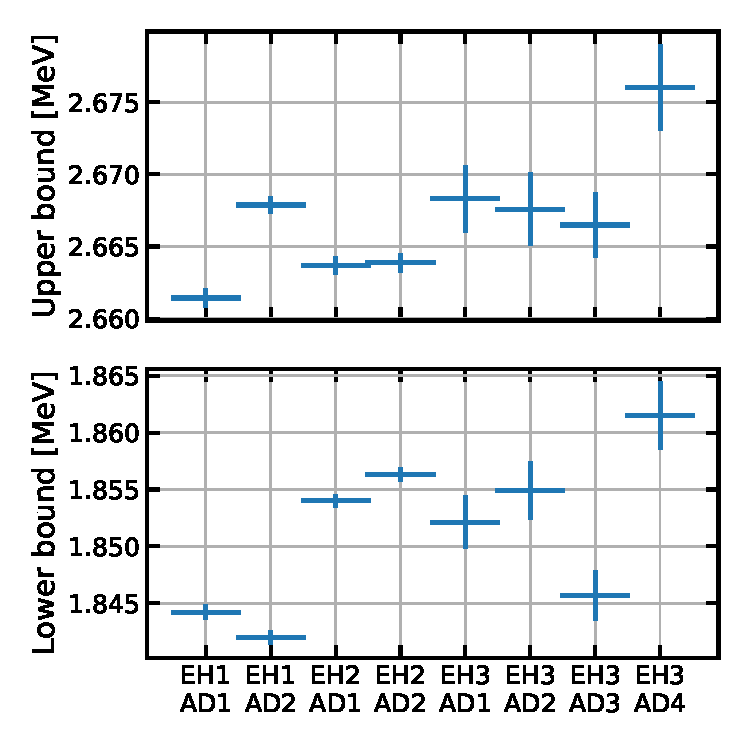
\includegraphics[height=0.40\textheight]{plot_diagnostics/delayed_energy_bounds.pdf}
    \caption{
        Delayed energy cut bounds computed as $\mu\pm 3\sigma$
        from the fitted histograms
    }
    \label{fig:delayed_bounds}
\end{figure}

The eight delayed energy spectra with their fits are shown in \cref{fig:delayed_fits}.
Comparing the fitted parameters across ADs can be used
to measure the identicalness of the ADs.
Their values and relative differences are plotted in \cref{fig:delayed_fit_parameters}
and listed in \cref{tab:delayed_fit_params}.
In particular, the top-left plot shows the relative difference
in the fitted peak $\mu$ across the ADs,
which is a measure of the energy scale variation.
The relative variation of \SI{+-0.5}{\percent}
is used to compute the AD-uncorrelated uncertainty
on the prompt energy cut efficiency.

The bounds for the delayed energy cut are computed
based on the fitted peak value and energy resolution
from the calorimter model. The energy criterion is

\begin{equation}
    \mu - 3\sigma < E < \mu + 3\sigma.
\end{equation}
This form was decided on even though the calorimeter function
is not symmetric, and even though in reality
the detector resolution changes with energy
(and therefore is not precisely modeled in the fit).
The values used for the energy bounds are listed in \cref{tab:delayed_bounds}
and plotted in \cref{fig:delayed_bounds}.

The absolute efficiency of the delayed energy cut
is measured using Monte Carlo.
The same fitting procedure with the calorimeter function
and the same $\mu \pm 3\sigma$ bounds are used to
estimate the fraction of neutron capture on hydrogen events
that pass the delayed energy cut.
The relative fraction of GdLS to LS also impacts the efficiency
because with more GdLS, fewer neutrons will capture on hydrogen.
This difference between the GdLS and LS regions is taken into account
when computing the absolute efficiency.

\begin{figure}
    \centering
    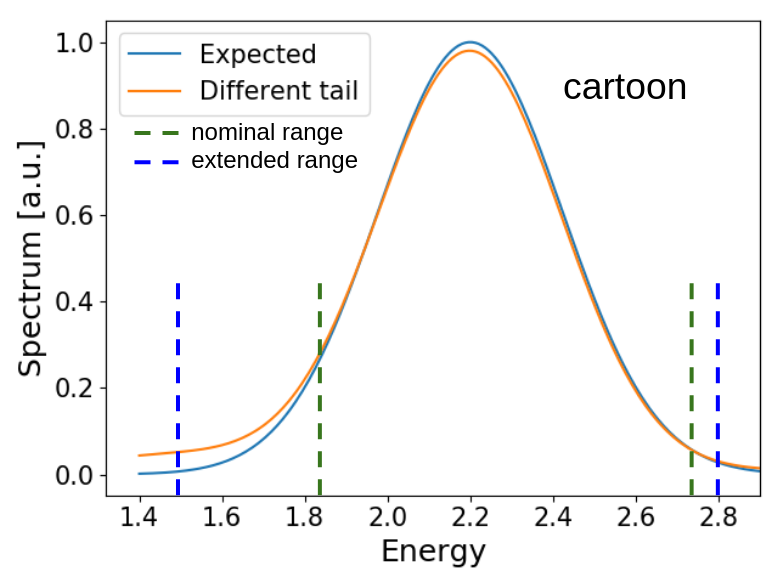
\includegraphics[height=0.4\textheight]{ch_event_selection/delayed_eff_uncertainty_cartoon}
    \caption{
        Intuition for how differences in the relative size
        of the nominal (peak) versus extended ranges
        are a proxy for differences in cut efficiency.
    }
    \label{fig:delayed_eff_unc_cartoon}
\end{figure}

The AD-uncorrelated uncertainty on the efficiency
includes variations due to all the above effects:
geometrical variations, energy scale, different material properties,
Gd fraction, etc.
The overall variation between ADs is estimated using a general method
that compares the relative size between the peak and tail regions
of the delayed energy spectrum, as defined by the delayed energy cut,
across the ADs.
Intuitively, if the same fraction of events is in the peak region in each AD,
then the cut efficiency must have a small variation.
This intuition is visualized in the cartoon in \cref{fig:delayed_eff_unc_cartoon}.
The ``expected'' curve has a high efficiency
and few events in the tail.
Since the ``different tail'' curve has more events in the tail region,
it can be concluded that this curve has a lower efficiency.

In practice, it is easier to compare the number of events in the peak
to the total number of events in an extended region that includes the tail,
rather than to just the new events in the tail.

For each AD's delayed energy spectrum, the peak region is defined as
the region passing the delayed energy cut, $\vert E-\mu \vert < 3\sigma$.
The extended region is the same for each AD:
$\SI{1.5}{\mev} < E < \SI{2.8}{\mev}$.
Using an AD-dependent definition for the peak region but
the same values for the extended creates
the desired sensitivity to variations in the energy scale.
Extending the lower bound down to \SI{1.5}{\mev} adds sensitivity to
anything that would change the shape of the tail
or the fraction of $\gamma$'s that (partially) escape from the AD.

\begin{figure}
    \centering
    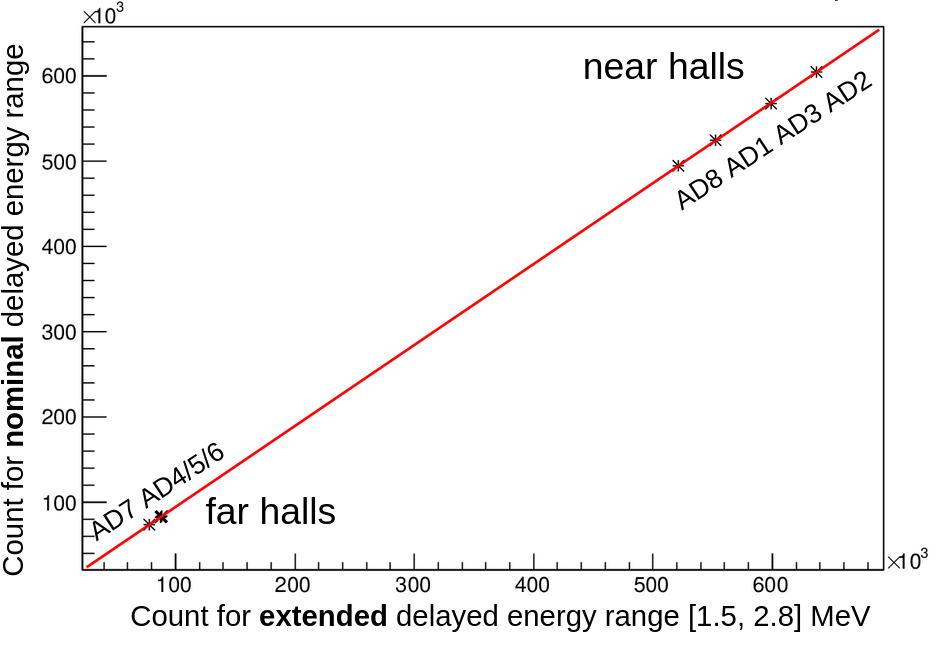
\includegraphics[height=0.4\textheight]{ch_event_selection/delayed_uncertainty_fit}\\
    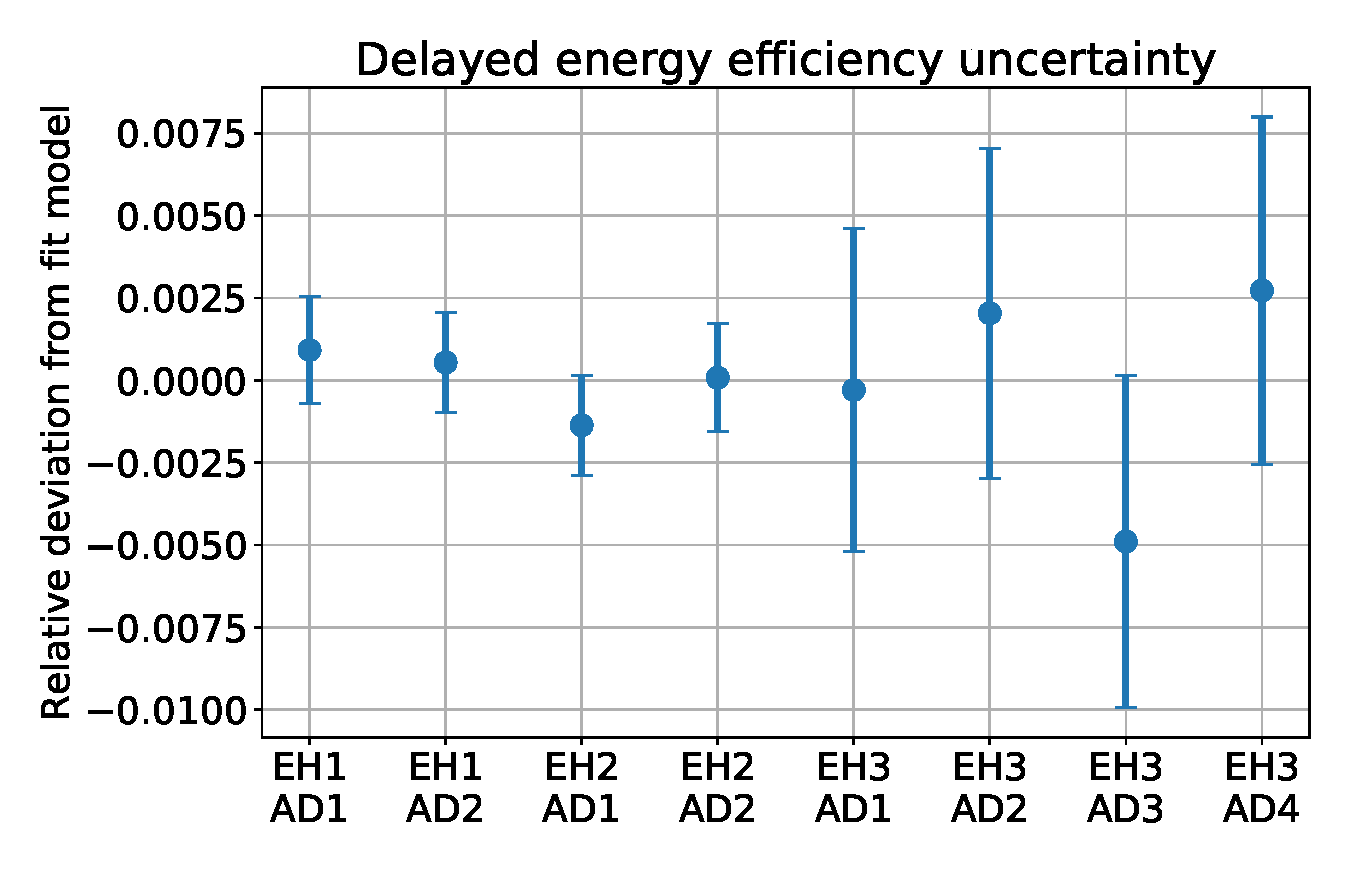
\includegraphics[height=0.4\textheight]{plot_diagnostics/delayed_energy_uncertainty_method1}
    \caption{
        (Top) Data points and (affine) linear fit
        to the number of events in the nominal (peak)
        and extended ranges of delayed energy.
        Statistical error bars are too small to be visible on this plot. \\
        (Bottom) Relative deviations from each hall to the fit model.
        The half-range of deviations for near-hall ADs
        is the delayed energy efficiency AD-uncorrelated uncertainty.
    }
    \label{fig:delayed_eff_unc_fit}
\end{figure}


If the delayed energy spectra have the same shape,
and if the calorimeter function is an appropriate fitting function
for determining the energy cut bounds,
then for some constant $b$ common to all ADs,
$N_{peak,\,i} = b N_{extended,\,i}$ for each AD $i$.
To test this model, an affine linear function is fit
to the values for each AD:

\begin{equation}
    N_{peak,\,pred,\,i} = a + b N_{extended,\,i},
\end{equation}
where $N_{peak,\,pred,\,i}$ is the fit function's prediction
of the actual event count in the peak ($N_{peak,\,i}$).
Plots of $N_{peak,\,i}$ vs. $N_{extended,\,i}$ and of the
relative deviation from the fitted line are shown in \cref{fig:delayed_eff_unc_fit}.
The fit value of $a$ should be $0$ if the simple model of
a linear scaling is correct.
Indeed, the fit value is $a = -321 \pm 387$
which is consistent with $0$.
The fit value for $b$ is $b = 0.9527 \pm 0.0015$,
which can be interpreted as a loose upper bound
on the delayed energy cut efficiency.
The final value for the AD-uncorrelated uncertainty
of the delayed energy efficiency is taken to be
the half-range of the relative deviations
of the near-hall ADs from the fitted line: \SI{0.11}{\percent}.
The far-hall ADs have much higher statistical uncertainty
(relative uncertainty $\approx\SI{0.5}{\percent}$),
and therefore larger fluctuations.
Validation that the far-hall ADs are not
substantially different from the near-hall ADs is obtained by
summing the counts for all 4 far-hall ADs to get
a combined relative deviation for the far hall of \SI{0.018}{\percent},
well within the uncertainty derived from the near halls.


